\documentclass[11pt]{article}
\usepackage[a4paper, total={6in, 8in}]{geometry}
\usepackage{amsmath}
\usepackage{amsthm}
\usepackage{graphicx}
\usepackage{amsfonts}
\usepackage{xcolor}
\begin{document}

\newtheorem{theorem}{Theorem}
\numberwithin{theorem}{section}
\theoremstyle{definition}
\newtheorem{definition}{Definition}
\newtheorem{proposition}{Proposition}
\newtheorem{example}{Example}
\newtheorem{lemma}{Lemma}
\newtheorem{corollary}{Corollary}
\numberwithin{definition}{section}
\numberwithin{proposition}{section}
\numberwithin{example}{section}
\numberwithin{lemma}{section}
\numberwithin{corollary}{section}
\newcommand{\uw}{\mathcal{U}(W,X)}
\newcommand{\W}{$(W,S)$}
\newcommand{\ix}{\textit}
\newcommand{\tr}{\textcolor{red}}
\newcommand{\sg}{$\Sigma$}


\title{Lectures on Buildings}
\maketitle
\tableofcontents 





\textcolor{red}{Red notes for Megan}

\textcolor{blue}{Blue notes for Yusra}

\section{Chamber systems}

\begin{definition}
    A set $C$ is called a \ix{chamber system} over a set $I$ if each $i\in I$ is an equivalence relation on the elements of $C$. Each $i$ partitions our set $C$. We say two elements $x,y\in C$ are \ix{i-adjacent}, and we write $x\sim_{i} y$, if they lie in the same part of the partition, i.e they are equivalent with respect to the equivalence relation corresponding to $i$. The elements of $C$ are called \ix{chambers}. The \ix{rank} of a chamber system is the size of $I$. 
\end{definition}


\tr{Other texts enforce that for each $i$ there are at least two elements which are $i$-adjacent.}


\begin{example}
    Given a group $G$, a subgroup $B$, and an indekxing set $I$, let there be a subgroup $B<P_i<G$ for all $i\in I$. Then we take as our chamber set $C$ the left cosets of $B$, and we define an equivalence relation
    \[gB\sim_{i}hB \textnormal{ if and only if }gP_i=hP_i.\]
\end{example}

\begin{definition}
    A finite sequence $(c_0,...,c_k)$ such that $c_i$ is adjacent to $c_{i+1}$ is called a \ix{gallery}. Its \ix{type} is a word $i_1,...,i_k$ in $I$ such that  $c_{i-1}$ is $i$-adjacent to $c_{i}$. We assume that no two consecutive chambers are equal.
\end{definition}

\begin{definition}
    We call $C$ \ix{connected} if we can connect any two chambers with a gallery. A \ix{J-residue} is a $J$-connected component. We call $\{i\}$-residues \ix{i-panels}. 
\end{definition}


\begin{definition}
    Let $C$ and $D$ be two chamber systems over the same indexing set $I$. A \ix{morphism} between $C$ and $D$ is a map $C\longrightarrow D$ which preserves $i$-adjacency.
\end{definition}

\subsection{The geometric realisation}

\begin{definition}
    Let $R$ be a $J$-residue and $S$ be a $K$-residue. Then $S$ is a \ix{face} of $R$ if $R\subset S$ and $J\subset K$. The \ix{cotype} of $J$ is the set $I-J$. 
\end{definition}


Observe that if $R$ is a residue of cotype $J$, we have
\begin{enumerate}
    \item for $K\subset J$, there is a unique face of $R$ which has cotype $K$.
    \item Let $S_1,S_2$ be faces of $R$ with cotypes $K_1$ and $K_2$. Then $S_1$ and $S_2$ have a shared face of cotype $K_1\cap K_2$. 
\end{enumerate}


With these observations, we can form a \ix{cell complex} of our chamber system. To do this, we form a vertex for each residue of corank 1. Then, we can associate to each residue of cotype $\{i,j\}$ an edge. From the observation above, this has as its boundary the residues of cotype $\{i\}$ and of cotype $\{j\}$. Then this can be continued inductively. 

\begin{definition}
    Let $\sigma$ be a simplex of our cell complex. The set \ix{star} $St(\sigma)$ is the corresponding residue. 
\end{definition}


\subsection{$A_n(k)$ Buildings}

Let us consider an $n+1$ dimensional vector space $V$ over a field $k$. We define the chambers of our chamber system to be the maximal sequences \[V_1\subset V_2\subset ...\subset V_n\] of subspaces of $V$, where $V_i$ has dimension $i$. We can then define adjancency by saying that two sequences $V_1\subset V_2\subset ...\subset V_n$ and $V_1'\subset V_2'\subset ...\subset V_n'$ are $i$-adjacent if and only if $V_j=v_j'$ for all $j\neq i$. Then the residues of type $i$ correspond to 1 spaces in the 2 space $V_{i+1}/V_{i-1}$. 

We then get a geometric realisation of this chmaber system. Here, a residue of cotype $J=\{j_1,...,j_r\}$ corresponds to a sequence \[V_{j_1}\subset V_{j_2}\subset ...\subset V_{j_r}.\] This residue has chambers which are maximal flags $V_1'\subset V_2'\subset ...\subset V_n'$ such that $V_j'=v_j$ if $j\in J$. 

In particular, residues of cotype $\{i\}$ correspond to the subspaces of $V$. 

\subsection{$C_n(k)$ Buildings}

........


\section{Coxeter Complexes}

Given a Coxeter group $W$, take as chambers the elements of $W$, and define an $i$-adjancency by $w\sim_iwr_i$, where $\{s_1,...,s_n\}$ are the set of generators of the Coxeter group. If the Coxeter group has Coxeter matrix $M$, we call this building a \ix{Coxeter complex of type M}.\\

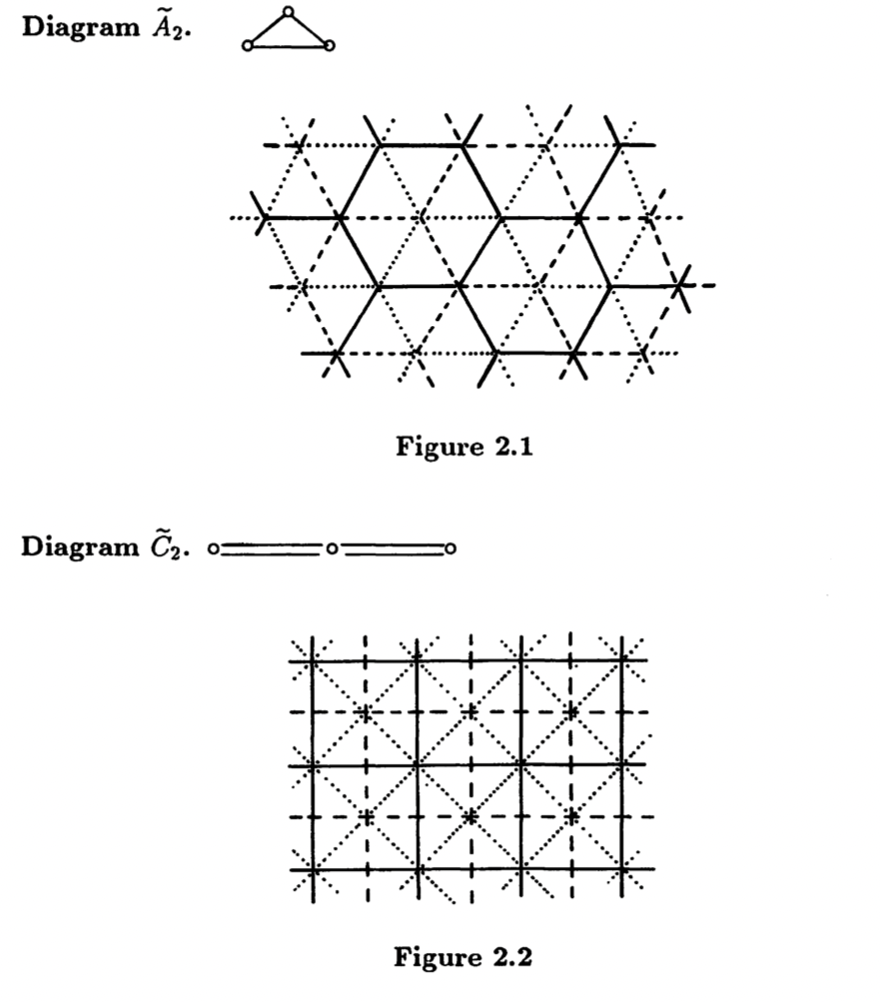
\includegraphics[scale=0.7]{Screenshot 2023-02-20 at 14.12.15.png}\\

\begin{lemma}
    The automorphism group of the Coxeter complex is isomorphic to the Coxeter group, and this acts simple-transitively on the set of chambers.
\end{lemma}

\begin{definition}
    A \ix{reflection r} of $W$ is a conjugate of the generators of $W$. The wall $M_r$ of a reflection $r$ is the set of simplicies in the Coxeter complex which is fied by $r$ when $r$ acts on the complex by left multiplication. Then $M_r$ is a subcomplex of codimension 1.
\end{definition}

\begin{theorem}
    There is a bijection between the set of reflections of a Coxeter group, and the set of walls in the corresponding Coxeter complex.
\end{theorem}

\begin{definition}
    A gallery $(c_0,...,c_k)$ \ix{crosses } $M_r$ if there is an $i$ such that $M_r$ interchanges $c_{i-1}$ and $c_i$. 
\end{definition}

\begin{lemma}
    \begin{enumerate}
        \item Any minimal gallery does not cross a wall twice.
        \item Every gallery from two alcoves $x$ and $y$ have the same parity of crossings of any wall.
    \end{enumerate}
\end{lemma}

\begin{definition}
    Each hyperplane splits an apartment into two half-apartments called \ix{roots}. If $\alpha$ is one root, we denote the other corresponding root by $-\alpha$. 
\end{definition}


\begin{definition}
    A set of alcoves is called \ix{convex} if any minimal gallery between two alcoves of the set lies entirely within the set. 
\end{definition}

\begin{proposition}
    \begin{enumerate}
        \item Roots are convex.
        \item Let $\alpha$ be a root, and let $x$ and $y$ be adjacent chambers with $x\in\alpha$ and $y\in -\alpha$. Then
        \[\alpha =\{c|d(x,c)<d(y,c)\}.\]
    \end{enumerate}
\end{proposition}










































































\end{document}